\documentclass{TDP005mall}

\usepackage{tabularx}
\usepackage{graphicx}
\usepackage{float}
\usepackage{csquotes}
\usepackage{mathtools}

\newcommand{\version}{Version 1.0}
\author{Jimmie Roos, \url{jimro697@student.liu.se}\\
  Sebastian Grunditz, \url{sebgr273@student.liu.se}}
\title{Kravspecifikation}
\date{2018-11-20}
\rhead{Jimmie Roos\\
Sebastian Grunditz}



\begin{document}
\projectpage
\section{Revisionshistorik}
\begin{table}[!h]
\begin{tabularx}{\linewidth}{|l|X|l|}
\hline
Ver. & Revisionsbeskrivning & Datum \\\hline
1.0 & Första utkast & 2018-11-20 \\\hline
\end{tabularx}
\end{table}


\section{Spelidé}
Spelet utspelas i en 2D-värld sett från sidan. Det går ut på att man ska döda bossar,
genom att skjuta eller slå på dem, så att deras health-bar töms. Efter att man dödat
en Boss erhåller man inte någon belöning i form av experience-points eller ny
utrustning. Detta gör så spelet belönar spelare som lär sig de spelmekaniker som finns,
istället för att de lutar sig på att utrustningen ska göra dem bättre.

Bossen kommer ha olika faser, som bestämmer vilka attacker och rörelsemönster den kommer ha.
Dessa faser bestäms av hur många livspoäng bossen har.

Ifall spelaren skulle dö, få slut på livspoäng innan bossens health-bar är tömd,
kommer fighten att startas om, och både spelare och boss återgår till fullt liv.

Level-designen kommer vara lite enklare, då det bara är meningen att faktiskt ha
mer komplicerad design under själva boss-fighterna. Under de fighterna ska banan
ha plattformar, som spelare och boss kan ställa sig på, samt en grundnivå, en \enquote{marknivå}.

Om tid finns, kommer ytterligare attacker för både spelare och boss läggas in, samt flera bossar.
Även ett system för att parera attacker kan läggas in, och då även ett system för
spelaren att återfå livspoäng.

\section{Målgrupp}
Spelet riktar sig mot personer som gillar utmanande spel som t.ex Dark Souls
eller Furi.

\section{Spelupplevelse}
Spelet ska vara oförlåtande och uppmuntra tålmodigt spelande då det inte finns
något enkelt sätt att få tillbaka health points när man väl tappat dom. Till en
början ska det kännas svårt men för varje försök så är tanken att man ska få
bättre koll på bossens attacker och på så sätt bli tillräckligt bra för att
döda bossen.

\section{Spelmekanik}
Menyer i spelet kontrolleras med W och S samt ENTER, och under spelets gång gäller följande kontroller:
\begin{table}[H]
\begin{tabularx}{\linewidth}{|l|p{14.39cm}|}
\hline
Tangent & Åtgärd \\\hline
A & Karaktären ska röra sig till vänster. \\\hline
D & Karaktären ska röra sig till höger. \\\hline
W & Karaktären rör sig uppåt i y-led på skärmen. \\\hline
S & Karaktären rör sig nedåt i y-led på skärmen om den står på en plattform. \\\hline
SPACE & Karaktären ska skjuta projektil. \\\hline
CTRL & Karaktären parerar en projektil. \\\hline
\end{tabularx}
\end{table}

\section{Regler}
\subsection{Spelplan}
Spelplanen består av en grundnivå som sträcker sig över hela skärmen. Både spelare
och boss ska kunna stå på denna grundnivå. Varken spelare eller boss ska kunna
röra sig utanför skärmens kanter. Utöver grundnivån, ska det finnas platformar,
som spelare och boss kan ställa sig på. Dessa kommer flyta i luften, och kan konfigureras
med en x-, och en y-koordinat.

\subsection{Spelare}
Spelaren ska kunna kollidera med väggar och plattformar. Spelaren ska inte kunna
röra sig utanför spelplanen. Vid kollision med boss eller projektil så ska
spelaren tappa livspoäng. Tappar spelaren alla sina livspoäng så ska game-over
meny visas med retry eller quit som menyval. Spelaren kan använda sitt
projektilvapen för att skada bossen. Spelaren kan även använda parering för att slå
tillbaka vissa typer av projektiler.

\subsection{Vapen och health bar}
\subsubsection{Projektiler}
Varken spelare eller boss har ett bestämt antal projektiler, utan har i princip
ett oändligt antal. Båda har dock ett max antal projektiler som får finnas på skärmen samtidigt.
Spelaren har 5 projektiler som max antal, medan bossen har olika max antal beroende
på vilken fas den är i och vilken boss det är.

Projektilerna från spelaren gör 10 skada. Projektilerna från bossen gör varierande
skada beroende på vilken attack som utförs. Bossens små projektiler gör 1 skada
medan de stora projektilerna gör 2.

När en projektil kommer i kontakt med spelaren eller bossen, samt om den åker utanför
skärmen, kommer den att förstöras.

\subsubsection{Parering}
Parering används av spelaren. Om en projektil är precis framför spelaren och
spelaren klickar på CTRL så ska projektilen skickas tillbaka till bossen och göra
lika mycket skada som en projektil från spelaren. Parering har ingen cooldown
så länge man lyckas med den, men om man skulle misslyckas så kan man ej använda
den på 2 sekunder.

\subsubsection{Health bar}
Spelaren har från början 10 livspoäng, som sedan går nedåt enligt attackernas skada på spelaren.

Bossarna har inkrementerande livspoäng, där den första bossen har lägst antal, och
den sista bossen har högst antal. Formeln för hur många livspoäng bossen har visas i
figur \ref{eq:1}.

\begin{equation} \label{eq:1}
  HP = 1000 + 10 * x^2
\end{equation}

X i figur \ref{eq:1} refererar till nuvarande boss-nivå, som är noll-indexerad.
Detta innebär att första bossen har 1000 livspoäng, andra bossen har 1010 livspoäng,
tredje har 1040, och så vidare. Detta lägger till ytterligare ett element till
svårighetsgraden i spelet.

\subsection{Fiendetyper}
\subsubsection{Boss}
Det finns en boss per fight. Bossen har livspoäng, attacker och skada baserat på
vilken nivå spelaren befinner sig på. Bossen kan ej röra sig utanför spelplanen.
\subsubsection{Summons}
Vissa bossar kommer att kalla på \enquote{summons}, små fiender som hjälper bossen
under stridens gång. Dessa kommer komma fram under vissa faser som dessa bossar har.
Det finns två sorters summons.
\begin{itemize}
  \item Jägare som rör sig mot spelaren.
  \item Skjutare som skjuter små projektiler, som kan pareras, mot spelaren.
\end{itemize}
Varje summon kan göra max 1 skada på spelaren, och dör av ett skott från spelaren.

\section{Visualisering}
\begin{\begin{figure}[H]
  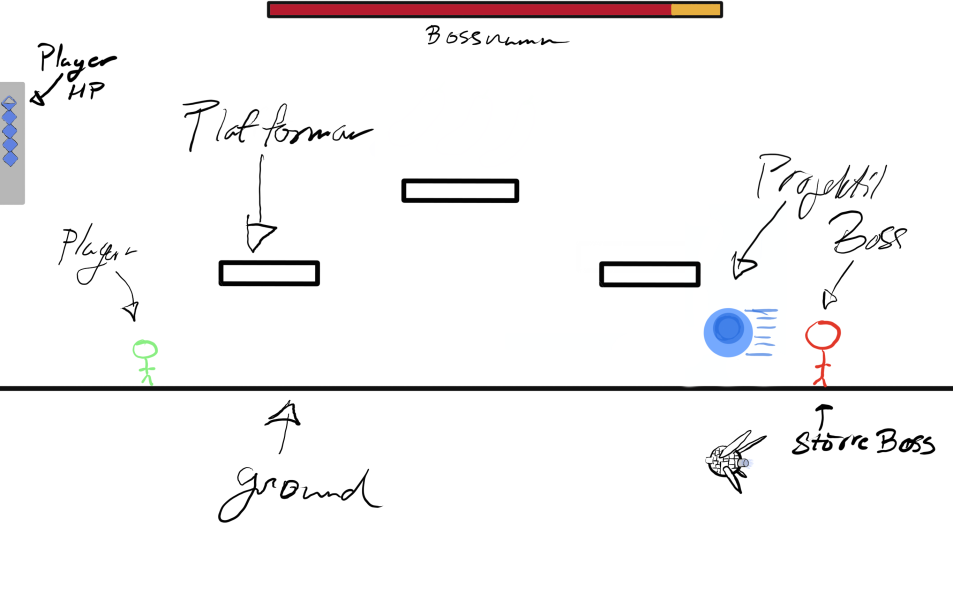
\includegraphics[width=\linewidth]{visualisering.png}
  \caption{Visualisering av spel.}
  \label{Fig:1}
\end{figure}}
\section{Kravformulering}
\subsection{Krav}
\begin{itemize}
  \item Spelet ska innehålla en spelare som styrs av oss.
  \item Spelet ska innehålla en boss som styrs av datorn.
  \item Spelet ska kunna hantera kollision mellan spelare och plattform/projektiler/boss.
  \item Spelare ska ha health bar.
  \item Bossen ska ha en health bar.
  \item Spelare ska kunna röra på sig.
  \item Spelare och bossen ska kunna skjuta projektiler.
  \item Spelarens health bar ska minska vid kollision med projektil eller boss.
  \item Bossens health bar ska minska vid kollision med projektil.
  \item Spelet ska innehålla en typ av projektil som både boss och spelare kan skjuta ut.
  \item Projektiler ska röra sig över skärmen, med ursprung från det objekt som sköt.
  \item En 2D-värld ska ritas ut lika stort som spelfönstret.
  \item Platformar i spelvärlden placeras ut genom att lägga till koordinater och storlek i en vector.
  \item Vectorn för platformar ska finnas i spel-loopen.
\end{itemize}

\subsection{Tilläggs-krav}
\begin{itemize}
  \item Spelaren ska kunnna parera projektiler.
  \item Parerade projektilers resevektor ska ändras så att de åker tillbaka dit de kom ifrån.
  \item Boss ska kunna kalla på hjälp i form av summons.
  \item Summons ska kunna skada spelaren med projektiler eller kollision med kropp.
  \item Det ska finnas fler nivåer med svårare bossar som blir starkare.
  \item Olika bossar ska ha olika skada och olika attacker.
\end{itemize}

\section{Kravuppfyllelse}
\subsection{Spelet ska simulera en värld som innehåller olika typer av objekt. Objekten ska ha olika beteenden och röra sig i världen och agera på olika sätt när de möter andra objekt.}
Uppfylls av krav 1, 3, 7, 8 och 9.
\subsection{Det måste finnas minst tre olika typer av objekt och det ska finnas flera instanser av minst två av dessa. T.ex ett spelarobjekt och många instanser av två olika slags fiendeobjekt.}
Uppfylls av krav 1, 4, 5 och 10.
\subsection{Ett beteende som måste finnas med är att figurerna ska röra sig över skärmen. Rörelsen kan följa ett mönster och/eller vara slumpmässig. Minst ett objekt, utöver spelaren ska ha någon typ av rörelse.}
Uppfylls av krav 6 och 11.
\subsection{En figur ska styras av spelaren, antingen med tangentbordet eller med musen. Du kan även göra ett spel där man spelar två stycken genom att dela på tangentbordet (varje spelare använder olika tangenter). Då styr man var sin figur.}
Uppfylls av krav 1.
\subsection{Grafiken ska vara tvådimensionell.}
Uppfylls av krav 12.
\subsection{Världen (spelplanen) kan antas vara lika stor som fönstret (du kan göra en större spelplan med scrollning, men det blir lite krångligare).}
Uppfylls av krav 12.
\subsection{Det ska finnas kollisionshantering, det vill säga, det ska hända olika saker när objekten möter varandra, de ska påverka varandra på något sätt. T.ex kan ett av objekten tas bort, eller så kan objekten förvandlas på något sätt, eller så kan ett nytt objekt skapas. (Ett exempel på att skapa/ta bort objekt är när man i Space Invaders trycker på skjuta-knappen, t.ex en musknapp, då avfyras ett laserskott och skottet blir då en ny figur som skapas och placeras i världen, på en position vid laserkanonens mynning. Skottet rör sig framåt (uppåt) och om det träffar ett fiendeskepp tas både skottet och skeppet bort, om skottet kommer utanför spelplanen, dvs det missar, tas det endast bort.)}
Uppfylls av krav 3, 8 och 9.
\subsection{Det ska vara enkelt att lägga till eller ändra banor i spelet. Detta kan exempelvis lösas genom att läsa in banor från en fil (lite som i Sokoban-labben i TDP002), eller genom att ha funktioner i programkoden som bygger upp en datastruktur som definierar en bana.}
Uppfylls av krav 13 och 14.
\subsection{Spelet måste upplevas som ett sammanhängande spel som går att spela!}
Uppfylls av alla krav.
\end{document}
